\documentclass[11pt]{article}
\usepackage{graphicx}
\usepackage[margin=1in]{geometry}
\usepackage{float}
\usepackage{amsmath,amssymb,times,mathptmx,subcaption,enumerate,fixltx2e,setspace,listings,textcomp,gensymb,relsize,multirow}
\usepackage[english]{babel}
\usepackage[titletoc]{appendix}
\usepackage{array}
\usepackage{fancyhdr}
\usepackage{tikz}
\usepackage{cancel}
\usepackage{subcaption}
\usepackage{algorithmic}
\usepackage{algorithm}
\renewcommand{\algorithmicrequire}{\textbf{Input:}}
\renewcommand{\algorithmicensure}{\textbf{Output:}}
\usetikzlibrary{shapes,arrows}
 \newcommand*\circled[1]{\tikz[baseline=(char.base)]{
            \node[shape=circle,draw,inner sep=0.8pt] (char) {#1};}}
\pagestyle{fancy}
\fancyhf{}
\rhead{\today}
\lhead{NPRE555 CP\#3\\
Longcong WANG}
\chead{Page \thepage}

\makeatletter
\newcommand*{\itemequation}[3][]{%
  \item
  \begingroup
    \refstepcounter{equation}%
    \ifx\\#1\\%
    \else  
      \label{#1}%
    \fi
    \sbox0{#2}%
    \sbox2{$\displaystyle#3\m@th$}%
    %\sbox4{\@eqnnum}%
    \dimen@=.5\dimexpr\linewidth-\wd2\relax
    % Warning for overlapping
    \ifcase
        \ifdim\wd0>\dimen@
          \z@
        \else
          \ifdim\wd4>\dimen@
            \z@
          \else 
            \@ne
          \fi 
        \fi
      \@latex@warning{Equation is too large}%
    \fi
    \noindent   
    \rlap{\copy0}%
    \rlap{\hbox to \linewidth{\hfill\copy2\hfill}}%
    \hbox to \linewidth{\hfill\copy4}%
    \hspace{0pt}% allow linebreak
  \endgroup
  \ignorespaces 
}
\makeatother  


\linespread{1}
\geometry{a4paper}
\setlength{\parskip}{0.5\baselineskip}
\setlength{\parindent}{0pt}

\begin{document}

% Define block styles
\tikzstyle{decision} = [diamond, draw, minimum width=4cm, 
    text width=4.5em, text badly centered, node distance=3cm, inner sep=0pt]
\tikzstyle{startstop} = [rectangle, draw, fill=blue!0, 
    text width=5em, text centered, rounded corners, minimum height=4em]
\tikzstyle{line} = [draw, -latex']
\tikzstyle{process} = [rectangle, minimum width=1cm, minimum height=1cm, 
text centered, draw=black]
\tikzstyle{io} = [trapezium, trapezium left angle=70, trapezium right angle=110, 
minimum width=1cm, minimum height=1cm, text centered, draw=black]
\begin{spacing}{1.5}
\title{NPRE 555 Computer Project 3 Report }
\author {Longcong WANG}
\date {\today}
\maketitle
\newpage
\tableofcontents
\listoffigures
\newpage
%---------------------------------------------------------------------------------------------------------
\section{$T_N$ Approximation}
In CP 2, the neutron transport equation was solved by $P_N$ approximation, which was shown to be a powerful method to get satisfactory results of slab reactor with isotropic scattering and source. However, it convergences slowly with anisotropic scattering \cite{anli2006tn}.To improve this, $T_N$ approximation which uses Chebyshev polynomials to replace Legendre polynomials is proposed. Most of previous studies focused on solving criticality problem using $T_N$ approximation. It is also shown that $T_N$ can be applied to eigenvalue spectrum and diffusion length calculation for bare and reflected slab or spheres \cite{okkecs2015diffusion}. In addition, $T_N$ approximation can be used for slab with strongly anisotropic scattering \cite{yilmazer2007solution} as well. However, for weak absorber, the result accuracy using $T_N$ method is not comparable to that using $P_N$ approximation \cite{anli2006tn}.\par
The basic idea of solving neutron transport problems using $T_N$ approximation method is expanding differential flux, cross section and neutron sources using Chebyshev polynomials \cite{anli2006tn}. Then, the transport equation can be simplified and solved by applying orthogonality and recurrence relation of Chebyshev polynomials. In this report, instead of criticality problem where $T_N$ approximation is widely used, the scalar neutron flux distribution in a 1-D slab reactor with isotropic scattering and isotropic source will be solved using $T_N$ approximation.\par

%---------------------------------------------------------------------------------------------------------
\section{Problem Description}
\subsection{Basic problem}
The problem solve in CP 2 using $P_N$ method is chosen as the basic problem. The flux distribution in a 1-D slab reactor with isotropic scattering and isotropic source will be solved using one-speed neutron transport equation. The entire domain is uniformly divided into $M-1$ cells and the material properties are summarized in Table. \ref{Material_properties}.
\begin{table}[!htbp]
\caption{Material properties of reactor}\label{Material_properties}
\centering
	\begin{tabular}{|c|c|}
		\hline
		$\Sigma_t$&0.17 $cm^{-1}$\\\hline
		$\Sigma_s$&0.10 $cm^{-1}$\\\hline
		$Q$ &10 $cm^{-3}s^{-1}$\\\hline

	\end{tabular}•
\end{table}•\par
The basic problem will be solved using $T_1$ approximation and the results will be compared with those evaluated using $P_1$ and $P_3$ approximation methods. 
%----------------------------------------------------------------------------------------------------------
\subsection{Challenging problems}
\subsubsection{Spatial convergence}
Spatial convergence will be conducted for $T_1$ approximation and the result will be used in hight order accuracy approximation. Initially, the entire domain is divided into 10 grid nodes and a initial guess of scalar flux $\phi_0$ distribution is obtained. Then, the mesh size will increase with increment of 1 and the relative error $\varepsilon$ will be compared to convergence criteria $\varepsilon_0$. If $\varepsilon\le\varepsilon_0$, the mesh is considered converged. $\varepsilon$ of mesh size $M+1$, $\varepsilon_{M+1}$, is defined as:
\[
\varepsilon_{M+1}=\frac{\left|\rm{avg}\left[\phi_0(M+1)\right]-\rm{avg}\left[\phi_0(M)\right]\right|}{\rm{avg}\left[\phi_0(M)\right]}
\]
\subsubsection{Order of accuracy convergence}
A general solution of $T_N$ approximation for 1-D slab reactor will be obtained. As is similar to $P_N$, only odd ordered $T_N$ approximations are considered. Then, the order of accuracy, $N$, will increase gradually with increment of $2$. The relative error $\varepsilon$ will be compared to the threshold $\varepsilon_0$, if $\varepsilon\le\varepsilon_0$, the result is considered converged. And $\varepsilon$ of $T_{N+2}$ approximation ($\varepsilon_{N+2}$) is defined as:
\[ 
\varepsilon_{N+2}\equiv\frac{\max\left|\phi_0(T_{N+2})-\phi_0(T_{N})\right|}{\phi_0(T_{N})}
\]
%--------------------------------------------------------------------------------------------------------
\section{Theory}
The one-dimensional neutron transport equation, for isotropic scattering and source, is:
\[
\mu\frac{d\psi(x,\mu)}{dx}+\Sigma_t\psi(x,\mu)=\frac{\Sigma_s}{2}\int^{1}_{-1}\psi(x,\mu')d\mu'+Q
\]
Expand $\psi(x,\mu)$ and $Q(x,\mu)$ using Chebyshev polynomials of first kind:
\[
\psi(x,\mu)=\frac{\phi_0(x)}{\pi\sqrt{1-\mu^2}}T_0(\mu)+\frac{2}{\pi\sqrt{1-\mu^2}}\sum_{n=1}^{N}\phi_n(x)T_n(\mu)
\]
\[
Q(x,\mu)=\frac{Q_0(x)}{\pi\sqrt{1-\mu^2}}T_0(\mu)+\frac{2}{\pi\sqrt{1-\mu^2}}\sum_{n=1}^{N}Q_n(x)T_n(\mu)
\]
$T_n$ are orthogonal with the weight $\frac{1}{\sqrt{1-x^2}}$ over the interval $[-1,1]$. Therefore, we have:
\[
\int_{-1}^1\frac{T_n(x)T_m(x)}{\sqrt{1-x^2}}dx=\begin{cases}
0&n\ne m\\
\pi&n=m=0\\
\frac{\pi}{2}&n=m\ne0
\end{cases}
\]
The recurrence relation of the Chebyshev polynomials of the first kind is:
\[
2\mu T_n(\mu)=T_{n+1}(\mu)+T_{n-1}(\mu)
\]
Using the orthogonality of $T_n$ and recurrence relation, the neutron transport equation can be written as:
\[
\frac{d\phi_1(x)}{dx}+\Sigma_t\phi_0(x)=\Sigma_s\phi_0(x)+Q_0(x)
\]
\[
\frac{d\phi_2(x)}{dx}+\frac{d\phi_0(x)}{dx}+2\Sigma_t\phi_1(x)=2Q_1(x)
\]
\[
\frac{d\phi_{n+1}(x)}{dx}+\frac{d\phi_{n-1}(x)}{dx}+2\Sigma_t\phi_n(x)=\frac{\left[1+(-1)^n\right]}{1-n^2}\Sigma_s\phi_0(x)+2Q_n(x),\quad n\ge2
\]
%------------------------------------------------------------------------------------------------------
\subsection{General equations}
For $T_{2N+1}$ approximation, $d\phi_{2N+2}/dx=0$. Therefore, for $n\ne 0$ and $n\ne2N+1$,
\[
\frac{d\phi_{n+1}(x)}{dx}+\frac{d\phi_{n-1}(x)}{dx}+2\Sigma_t\phi_n(x)=\frac{\left[1+(-1)^n\right]}{1-n^2}\Sigma_s\phi_0(x)+2Q_n(x),\quad n\ge2
\]
where:
\[
\phi_n(x)=\int_{-1}^{1}\psi(x,\mu)T_n(\mu)d\mu
\]
\[
Q_n(x)=\int_{-1}^{1}Q(x,\mu)T_n(\mu)d\mu
\]

If we introduce new set of variables $F_n$ for $T_{2N+1}$ approximation ($N\ge1$) and define:
\[
F_N=\phi_{2N}
\]
\[
F_n=\phi_{2n}+\phi_{2n+2}
\]
The odd ordered $T_n$ equation gives:
\[
\begin{aligned}
\phi_{2n+1}(x)&=\frac{1}{2\Sigma_t}\left[2Q_{2n+1}(x)-\frac{d\phi_{2n+2}(x)}{dx}-\frac{d\phi_{2n}(x)}{dx}\right]\\
&=\frac{1}{2\Sigma_t}\left[2Q_{2n+1}(x)-\frac{dF_{n}(x)}{dx}\right]
\end{aligned}
\]
Plug $\phi_{2n+1}(x)$ and $\phi_{2n-1}(x)$ into $2n_{th}$ ordered $T_n$ equation:
\[
\frac{d}{dx}\left\{\frac{1}{2\Sigma_t}\left[2Q_{2n+1}(x)-\frac{dF_{n}(x)}{dx}\right]\right\}+\frac{d}{dx}\left\{\frac{1}{2\Sigma_t}\left[2Q_{2n-1}(x)-\frac{dF_{n-1}(x)}{dx}\right]\right\}+2\Sigma_t\phi_{2n}(x)=\frac{2\Sigma_s}{1-4n^2}\phi_0(x)+2Q_{2n}(x)
\]
And
\[
\phi_{2n}=F_n-F_{n+1}+F_{n+2}\dots=\sum_{m=0}^{N-n}(-1)^{m}F_{n+m}
\]
For isotropic source and scattering:
\[
Q_{2n+1}=Q_{2n-1}=0
\]
\begin{equation}\label{GE1}
\boxed{
-\frac{d^2F_{n}(x)}{dx^2}-\frac{d^2F_{n-1}(x)}{dx^2}+4\Sigma_t^2\sum_{m=0}^{N-n}(-1)^{m}F_{n+m}(x)=\frac{4\Sigma_s\Sigma_t}{1-4n^2}\sum_{m=0}^{N}(-1)^{m}F_{m}+4\Sigma_tQ_{2n}(x)
}
\end{equation}
Then, we can reduce the number of variables from $2N+2$ to $N+1$. Discretizing Eq \ref{GE1}:
\begin{equation}
\boxed{
-\frac{F_n^{i-1}-2F_n^{i}+F_n^{i+1}}{\Delta x^2}-\frac{F_{n-1}^{i-1}-2F_{n-1}^{i}+F_{n-1}^{i+1}}{\Delta x^2}+4\Sigma_t^2\sum_{m=0}^{N-n}(-1)^{m}F_{n+m}^i-\frac{4\Sigma_s\Sigma_t}{1-4n^2}\sum_{m=0}^{N}(-1)^{m}F_{m}^i=4\Sigma_tQ_{2n}^i
}
\end{equation}•
%---------------------------------------------------------------------------------------------------------
\subsection{Special cases}
If $n=0$,
\[
\boxed{
-\frac{d^2F_{0}(x)}{dx^2}+2\Sigma_t^2\sum_{m=0}^{N}(-1)^{m}F_{m}(x)=2\Sigma_s\Sigma_t\sum_{m=0}^{N}(-1)^{m}F_{m}+2\Sigma_tQ_{0}(x)
}
\]
%---------------------------------------------------------------------------------------------------------
\subsection{Solution}
Therefore, $F_n(x)$ of $T_{2N+1}$ approximation with $M$ grid nodes can be obtained by solving the following linear algebra system:
\[
\mathbf{A}\mathbf{F}=\mathbf{Q}
\]
where $\mathbf{A}$ is the coefficient matrix with size $(N+1)M\times(N+1)M$, $\mathbf{F}=[f_0,f_1,\dots f_{(N+1)M-1}]^T$ is the vector of neutron fluxes and $\mathbf{Q}=[Q_0,Q_1,\dots Q_{(N+1)M-1}]$. And
\[
f_{nM+i}=F_n^{i}
\]
\[
Q_{nM+i}=4\Sigma_tQ_{2n}^i
\]

%----------------------------------------------------------------------------------------------------------
\subsection{Marshak Boundary Condition}
The Marshak boundary conditions are given as:
\[
\int_{0}^{1}\psi(0,\mu)T_k(\mu)d\mu=0,\quad k=1,3,5,\dots,N.
\]
\[
\int_{-1}^{0}\psi(a,\mu)T_k(\mu)d\mu=0,\quad k=1,3,5,\dots,N.
\]
This type of B.C. yields:
\begin{equation}\label{Marshak1}
H_k\phi_0(0)+\sum^{2N+1}_{n=1}H_{n,k}\phi_n(0)=0
\end{equation}
\begin{equation}\label{Marshak2}
I_k\phi_0(a)+\sum^{2N+1}_{n=1}I_{n,k}\phi_n(a)=0
\end{equation}
where:
\[
H_k=\int_0^1\frac{T_k(\mu)}{\sqrt{1-\mu^2}}d\mu=\begin{cases}
\pi/2&k=0\\
\frac{\sin(k\pi/2)}{k}&k\ge1
\end{cases}
\]
\[
H_{n,k}=\int_0^1\frac{2T_k(\mu)T_n(\mu)}{\sqrt{1-\mu^2}}d\mu=\begin{cases}
\pi/2&n=k\ne 0\\
\frac{\sin((n+k)\pi/2)}{(n+k)}+\frac{\sin((n-k)\pi/2)}{(n-k)}&n\ne k
\end{cases}
\]
\[
I_k=\int_{-1}^0\frac{T_k(\mu)}{\sqrt{1-\mu^2}}d\mu=\begin{cases}
\pi/2&k=0\\
-\frac{sin(k\pi/2)}{k}&k\ge1
\end{cases}
\]
\[
I_{n,k}=\int_{-1}^0\frac{2T_k(\mu)T_n(\mu)}{\sqrt{1-\mu^2}}d\mu=\begin{cases}
\pi/2&n=k\ne 0\\
-\frac{\sin[(n+k)\pi/2]}{(n+k)}-\frac{\sin[(n-k)\pi/2]}{(n-k)}&n\ne k
\end{cases}
\]
It is noticed that $k$ only takes odd number, so for odd $n$, $I_{n,k}=0$, if $n\ne k$. Only even ordered $\phi_n$ are left in Eq. \ref{Marshak1} and \ref{Marshak2}.\par
If $k=2m+1$ and $n=2a$,
\[
H_{2m+1}=\int_0^1\frac{T_{2m+1}(\mu)}{\sqrt{1-\mu^2}}d\mu=\frac{(-1)^m}{2m+1}
\]
\[
H_{2a,2m+1}=\int_0^1\frac{2T_{2m+1}(\mu)T_{2a}(\mu)}{\sqrt{1-\mu^2}}d\mu=
\frac{(-1)^{a+m}}{2a+2m+1}+\frac{(-1)^{a-m+1}}{2a-2m-1}
\]
\[
I_{2m+1}=\int_{-1}^0\frac{T_{2m+1}(\mu)}{\sqrt{1-\mu^2}}d\mu=
\frac{(-1)^{m+1}}{2m+1}
\]
\[
I_{2a,2m+1}=\int_{-1}^0\frac{2T_{2m+1}(\mu)T_{2a}(\mu)}{\sqrt{1-\mu^2}}d\mu=
\frac{(-1)^{a+m+1}}{2a+2m+1}+\frac{(-1)^{a-m}}{2a-2m-1}
\]
For odd\textsuperscript{th} ordered $\phi_{2n+1}$ at left boundary:
\[
\begin{aligned}
\phi_{2n+1}(0)&=-\frac{1}{H_{2n+1,2n+1}}\left\{H_{2n+1}\sum_{m=0}^{N}(-1)^{m}F_{m}(0)+\sum_{a=1}^{N}H_{2a,2n+1}\sum_{m=0}^{N-a}(-1)^{m}F_{a+m}(0)\right\}\\
&=\frac{1}{2\Sigma_t}\left[2\cancelto{0}{Q}_{2n+1}-\frac{dF_{n}(0)}{dx}\right]=-\frac{1}{2\Sigma_t}\frac{dF_{n}(0)}{dx}
\end{aligned}
\]
Using ghost nodes at left boundary, 
\[
\frac{1}{2\Sigma_t}\frac{F_{n}^1-F_{n}^{-1}}{\Delta x}=\frac{1}{H_{2n+1,2n+1}}\left\{H_{2n+1}\sum_{m=0}^{N}(-1)^{m}F_{m}^1+\sum_{a=1}^{N}H_{2a,2n+1}\sum_{m=0}^{N-a}(-1)^{m}F_{a+m}^1\right\}
\]
\[
\boxed{
\Longrightarrow F_n^{-1}=F_n^1-\frac{2\Sigma_t\Delta x}{H_{2n+1,2n+1}}\left\{H_{2n+1}\sum_{m=0}^{N}(-1)^{m}F_{m}^0+\sum_{a=1}^{N}H_{2a,2n+1}\sum_{m=0}^{N-a}(-1)^{m}F_{a+m}^0\right\}
}
\]
where $F_n^{-1}$ denotes the ghost point outside the entire domain.
Similarly, at right boundary:
\[
\begin{aligned}
\phi_{2n+1}(a)&=-\frac{1}{I_{2n+1,2n+1}}\left\{I_{2n+1}\sum_{m=0}^{N}(-1)^{m}F_{m}(a)+\sum_{a=1}^{N}I_{2a,2n+1}\sum_{m=0}^{N-a}(-1)^{m}F_{a+m}(a)\right\}\\
&=\frac{1}{2\Sigma_t}\left[2\cancelto{0}{Q}_{2n+1}-\frac{dF_{n}(a)}{dx}\right]=-\frac{1}{2\Sigma_t}\frac{dF_{n}(a)}{dx}
\end{aligned}
\]
\[
\boxed{
\Longrightarrow F_n^{M}=F_n^{M-2}+\frac{2\Sigma_t\Delta x}{I_{2n+1,2n+1}}\left\{I_{2n+1}\sum_{m=0}^{N}(-1)^{m}F_{m}^{M-1}+\sum_{a=1}^{N}I_{2a,2n+1}\sum_{m=0}^{N-a}(-1)^{m}F_{a+m}^{M-1}\right\}
}
\]
%-----------------------------------------------------------------------------------------------------------
\subsection{$T_1$ approximation}
For $T_1$ approximation, only $F_0$ exists:
\[
-\frac{d^2F_{0}(x)}{dx^2}+2\Sigma_t^2F_{0}(x)=2\Sigma_s\Sigma_tF_{0}(x)+2\Sigma_tQ_{0}(x)
\]
\[
-\frac{F_0^{i-1}-2F_0^i+F_0^{i+1}}{\Delta x^2}+2\Sigma_t^2F_{0}^i-2\Sigma_s\Sigma_tF_{0}^i=2\Sigma_tQ_{0}(x)
\]
The Marshak boundary conditions give:
\[
\phi_0(0)+\frac{\pi}{2}\phi_1(0)=F_0(0)-\frac{\pi}{4\Sigma_t}\frac{dF_0(0)}{dx}=0
\]
\[
-\phi_0(a)+\frac{\pi}{2}\phi_1(a)=-F_0(a)-\frac{\pi}{4\Sigma_t}\frac{dF_0(a)}{dx}=0
\]
\[
F_0^0-\frac{\pi}{4\Sigma_t}\frac{F_0^1-F_0^{-1}}{\Delta x}=0\Longrightarrow F_0^{-1}=F_0^1-\frac{4\Delta x\Sigma_t}{\pi}F_0^0
\]
\[
-F_0^{M-1}-\frac{\pi}{4\Sigma_t}\frac{F_0^M-F_0^{M-2}}{\Delta x}=0\Longrightarrow F_0^{M}=F_0^{M-2}-\frac{4\Delta x\Sigma_t}{\pi}F_0^{M-1}
\]
Then, for $1\le n\le M-2$:
\[
A[n,n]=\frac{2}{\Delta x^2}+2\Sigma_t^2-2\Sigma_s\Sigma_f
\]
\[
A[n,n-1]=A[n,n+1]=-\frac{1}{\Delta x^2}
\]
At boundaries:
\[
A[0,0]=A[M-1,M-1]=\frac{2}{\Delta x^2}+2\Sigma_t^2-2\Sigma_s\Sigma_f+\frac{4\Sigma_t}{\pi\Delta x}
\]
\[
A[0,1]=A[M-1,M-2] = -\frac{2}{\Delta x^2}
\]
The source terms are given as:
\[
Q[n]=2\Sigma_tQ_0=2\Sigma_tQ
\]
\newpage
%--------------------------------------------------------------------------------------------------------------
\section{Results \& Discussion}
\subsection{Basic problem}
The basic problem is solving using $T_1$ approximation and the result of scalar flux is shown and compared with results of $P_1$ and $P_3$ approximations in Fig. \ref{fig:basic}. In general, scalar fluxes obtained using $T_1$, $P_1$ and $P_3$ approximations follow the same pattern. In the middle of slab, the flux is almost constant. In this region, $T_N$ and $P_N$ agree perfectly with each other. Near boundaries, $T_1$ approximation behaviors similarly as $P_3$ approximation. However, in the shoulder region, the fluxes evaluated using $T_1$ and $P_1$ approximations are almost identical. 
\begin{figure}[htbp]
\centering
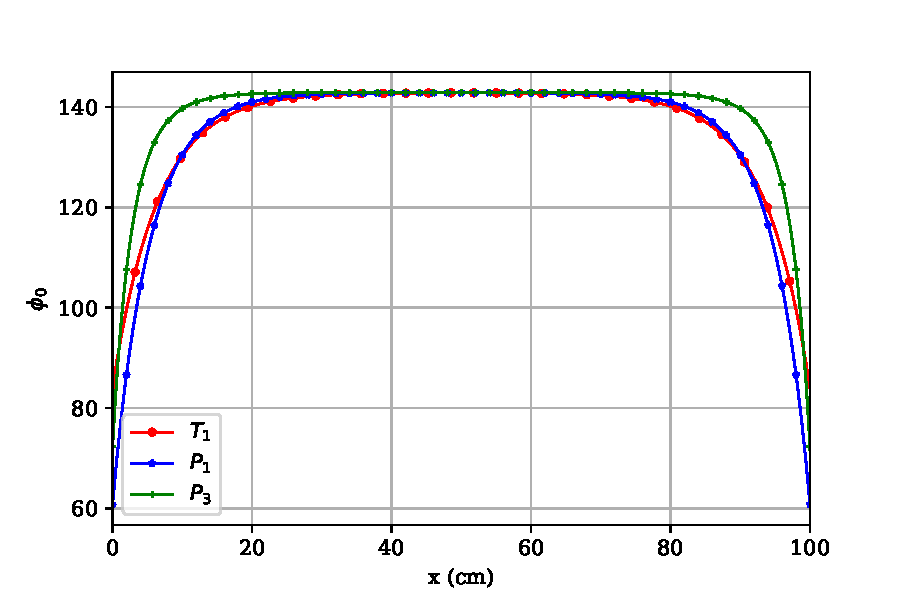
\includegraphics{TP_comp_2.pdf}
\caption{Comparison of $T_N$ and $P_N$ methods}\label{fig:basic}
\end{figure}•
%-------------------------------------------------------------------------------------------------------------
\subsection{Challenging problems}
\subsubsection{Spatial convergence}
 The change of relative error $\varepsilon$ with mesh size increasing is summarized in Fig. \ref{fig:spa_conv}. The threshold $\varepsilon_0$ is set to be $1\times10^{-6}$ and the refined mesh size is 619. It is shown that $\varepsilon$ monotonically decreases as mesh becomes more refined. And it decreases more slowly as mesh size increases. 
\begin{figure}[htbp]
\begin{minipage}[t]{0.5\textwidth}
\centering
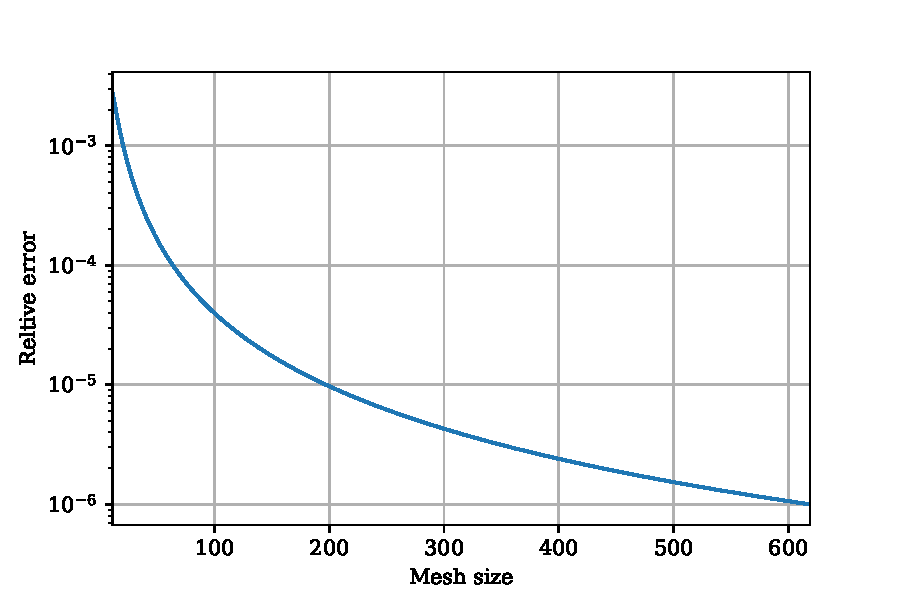
\includegraphics[width=3in]{conv_mesh_2.pdf}
\caption{Spatial convergence}\label{fig:spa_conv}
\end{minipage}
\begin{minipage}[t]{0.5\textwidth}
\centering
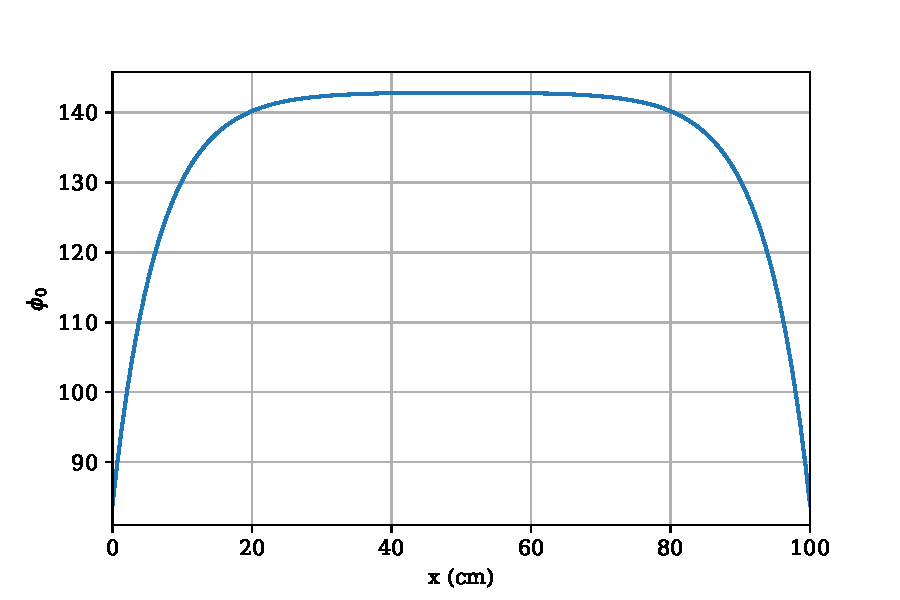
\includegraphics[width=3in]{T1_final_2.pdf}
\caption{Converged scalar flux with $T_1$ approximation}
\end{minipage}
\end{figure}•
%-------------------------------------------------------------------------------------------------------------
\subsubsection{Order of accuracy convergence}
After conducting spatial convergence, influence of order of accuracy on the results are studied by changing the order of $T_N$ approximation incrementally. The convergence criteria $\varepsilon_0=1\times10^{-3}$. The results of order of accuracy convergence are summarized in Fig. \ref{fig:order_conv}. The converged scalar flux is plotted in Fig. \ref{fig:conv_flux} and compared with lower order of accuracy in Fig. \ref{fig:comp_final}. Based on Fig. \ref{fig:comp_final}, in general, $\varepsilon$ decreases as order of accuracy increases. However, error does not change monotonically. On the contrary, it decreases jaggedly as higher ordered approximation is made.\par
In summary, $T_{23}$ approximation is sufficient to provide satisfactory solutions of neutron transport equation. Based on Fig. \ref{fig:comp_final}, the finally converged result is located between results from $P_1$ and $P_3$ approximations. It is closer to $P_3$ approximation than $P_1$ approximation. It can be noticed that solutions of $T_{11}$ and $T_{23}$ are almost identical. However, the computational power needed continuous to increases as the order of accuracy becomes higher. Therefore, further increases of order of accuracy do not benefit much. 
\begin{figure}[htbp]
\begin{minipage}[t]{0.5\textwidth}
\centering
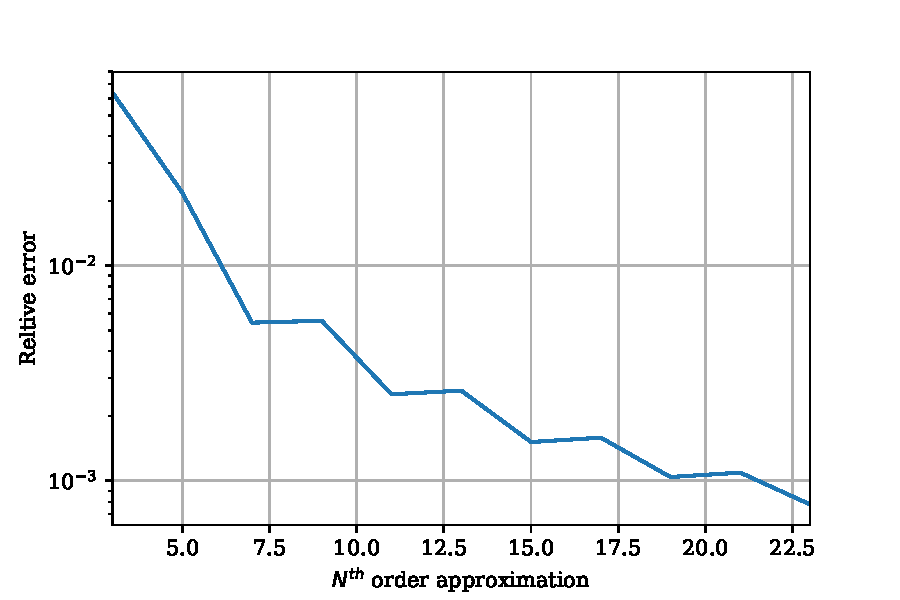
\includegraphics[width=3in]{order_conv_2.pdf}
\caption{Order of accuracy convergence}\label{fig:order_conv}
\end{minipage}
\begin{minipage}[t]{0.5\textwidth}
\centering
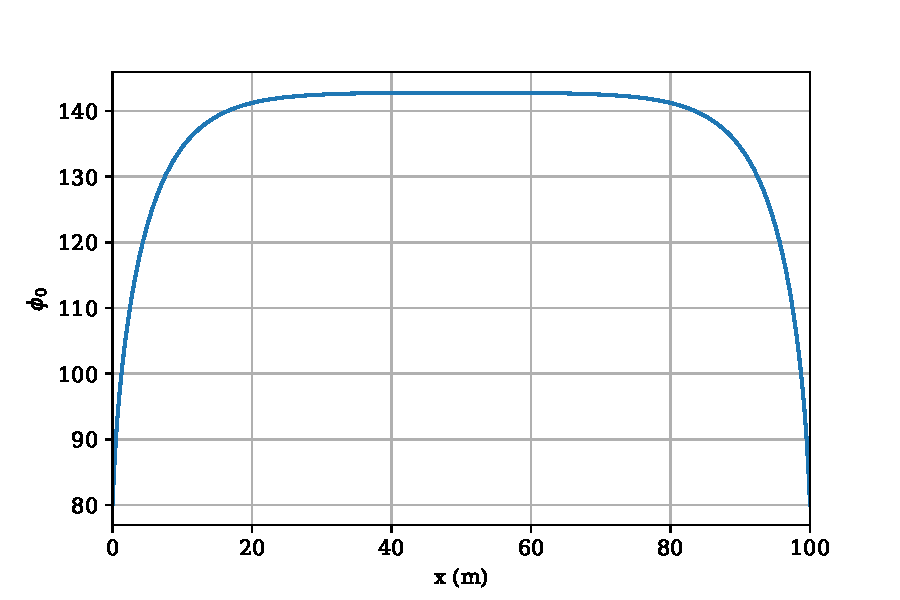
\includegraphics[width=3in]{phi0_final_2.pdf}
\caption{Converged scalar flux}\label{fig:conv_flux}
\end{minipage}
\end{figure}•
\begin{figure}[htbp]
\centering
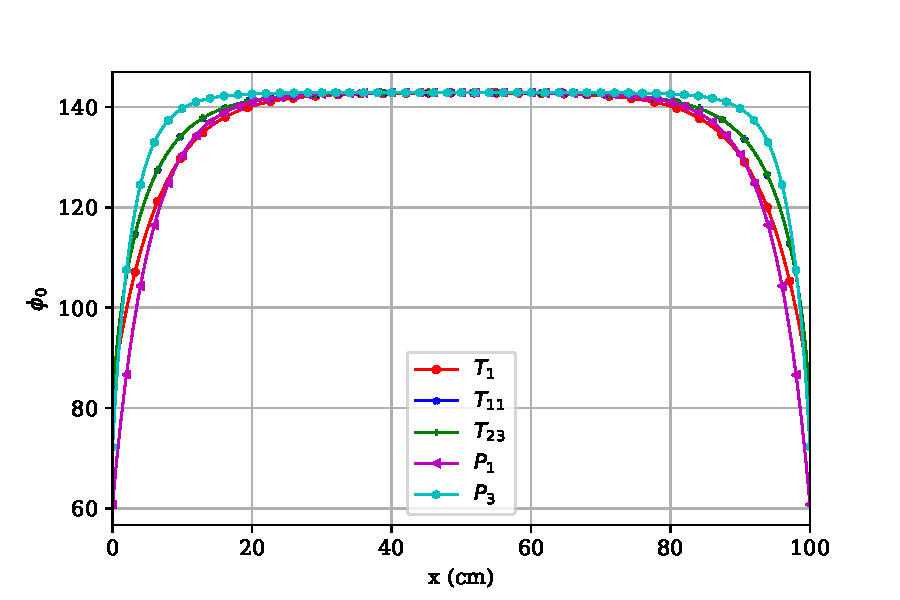
\includegraphics{TP_comp_final_2.pdf}
\caption{Comparison of $T_N$ and $P_N$ methods after convergence studies}\label{fig:comp_final}
\end{figure}•
%-------------------------------------------------------------------------------------------------------------
\section{Conclusion}
In conclusion, $T_N$ approximation method can be a powerful tool to solve one-speed neutron transport equation in 1-D slab. It can be roughly concluded that results of $T_N$ approximation  agree with those of $P_N$ approximation. However, required computational power and computer memory increase dramatically as the order of accuracy increase, even for the simplest 1-D problem. Therefore, the algorithm and code should be improved to apply to complex geometries and multi-group problems.
\newpage
%-----------------------------------------------------------------------------------------------------------
\bibliographystyle{plain}
\bibliography{bib}

\end{spacing}
\end{document}